% CVPR 2023 Paper Template
% based on the CVPR template provided by Ming-Ming Cheng (https://github.com/MCG-NKU/CVPR_Template)
% modified and extended by Stefan Roth (stefan.roth@NOSPAMtu-darmstadt.de)

\documentclass[10pt,twocolumn,letterpaper]{article}

%%%%%%%%% PAPER TYPE  - PLEASE UPDATE FOR FINAL VERSION
\usepackage[review]{cvpr}      % To produce the REVIEW version
%\usepackage{cvpr}              % To produce the CAMERA-READY version
%\usepackage[pagenumbers]{cvpr} % To force page numbers, e.g. for an arXiv version

% Include other packages here, before hyperref.
\usepackage{graphicx}
\usepackage{amsmath}
\usepackage{amssymb}
\usepackage{booktabs}


% It is strongly recommended to use hyperref, especially for the review version.
% hyperref with option pagebackref eases the reviewers' job.
% Please disable hyperref *only* if you encounter grave issues, e.g. with the
% file validation for the camera-ready version.
%
% If you comment hyperref and then uncomment it, you should delete
% ReviewTempalte.aux before re-running LaTeX.
% (Or just hit 'q' on the first LaTeX run, let it finish, and you
%  should be clear).
\usepackage[pagebackref,breaklinks,colorlinks]{hyperref}


% Support for easy cross-referencing
\usepackage[capitalize]{cleveref}
\crefname{section}{Sec.}{Secs.}
\Crefname{section}{Section}{Sections}
\Crefname{table}{Table}{Tables}
\crefname{table}{Tab.}{Tabs.}


%%%%%%%%% PAPER ID  - PLEASE UPDATE
\def\cvprPaperID{*****} % *** Enter the CVPR Paper ID here
\def\confName{CVPR}
\def\confYear{2023}


\begin{document}

%%%%%%%%% TITLE - PLEASE UPDATE
%\title{\LaTeX\ Author Guidelines for \confName~Proceedings}
\title{D-Gait: A Dataset for Auxiliary Depression Diagnosis based on Gait}

\author{First Author\\
Institution1\\
Institution1 address\\
{\tt\small firstauthor@i1.org}
% For a paper whose authors are all at the same institution,
% omit the following lines up until the closing ``}''.
% Additional authors and addresses can be added with ``\and'',
% just like the second author.
% To save space, use either the email address or home page, not both
\and
Second Author\\
Institution2\\
First line of institution2 address\\
{\tt\small secondauthor@i2.org}
}
\maketitle

%%%%%%%%% ABSTRACT
\begin{abstract}
   The ABSTRACT is to be in fully justified italicized text, at the top of the left-hand column, below the author and affiliation information.
   Use the word ``Abstract'' as the title, in 12-point Times, boldface type, centered relative to the column, initially capitalized.
   The abstract is to be in 10-point, single-spaced type.
   Leave two blank lines after the Abstract, then begin the main text.
   Look at previous CVPR abstracts to get a feel for style and length.
\end{abstract}

%%%%%%%%% BODY TEXT
\section{Introduction}
\label{sec:intro}

Mental illness is one of the most important diseases of people, and depression is the most common psychological disease ~\cite{world2017depression,bhugra2004globalisation,rao2008understanding}.
According to World Health Organization (WHO), the cases of depression is rising by more than 25\% around the world during Covid-19. With the increase of academic stress and social pressure, the age of depressed people is becoming younger and younger. Many teenagers suffer from depression, which seriously affects the health of teenagers and their families.
Although suffering from depression does not directly lead to death, but many Major Depressive Disorder (MDD) people have the suicide tendency~\cite{eisenberg2007prevalence,bergfeld2018treatment,hemming2019alexithymia}.
In statistical surveys, the probability of suicide in depressed people is around 10-15\%, which has great impact on personal wellbeing and social stability.

%-------------------------------------------------------------------------
%\subsection{Language}

%{\bf There will be no extra page charges for \confName\ \confYear.}

Because of the high prevalence of depression and high suicide rate, it is becoming increasingly important to have an effective diagnostic protocol to detect depression. However, the clinical diagnosis of depression is cumbersome. People should go to designated hospitals or clinics, and professional doctors need to make comprehensive judgments based on disease history, clinical symptoms, degree of disease, physical condition and laboratory tests~\cite{faust1988expert}. Moreover, some people are resistant and do not cooperate with diagnosis or treatment, which missing the best time for treatment.


%-------------------------------------------------------------------------

\begin{figure}[t]
  \centering
  %\fbox{\rule{0pt}{2in} \rule{0.9\linewidth}{0pt}}
   \includegraphics[width=1.0\linewidth]{figures/example.png}

   \caption{Example of dataset: Different gait representations of the same person from multiple cameras and clothes.
   The rows show subject with multiple views from different cameras. The columns show subject with 3 different clothes.
   }
   \label{Introduction}
\end{figure}

%-------------------------------------------------------------------------
%\subsection{The ruler}

The gait of person is stable, and it’s difficult to disguise or change. Many researches shows that the fluctuations in mood can lead the changes in gait specially in some gait characteristics, such as the number of arm swings, stride length and walking speed~\cite{hicheur2013perception,montepare1987identification,roether2009critical,venture2014recognizing,gross2012effort,janssen2008recognition,kang2016effect,li2016emotion,li2016identifying,bhattacharya2020step} .
Negative emotions are the basic manifestation in depressed people, and research showed that the analysis of abnormal gait can also be applied to the recognition of depression ~\cite{michalak2009embodiment}. People with depression will be accompanied by decreased vertical head movement, reduced limb range of motion, and slower pace ~\cite{sloman1982gait,lemke2000spatiotemporal,bovi2011multiple,radovanovic2014gait,zhao2019see,yuan2018depression,fang2019depression,jing2019different}.
Compared with traditional psychological measurement methods, the mental disease identification method based on gait data has the advantages of non-interference, traceability, automation and so on, which can effectively improve the accuracy of mental disease detection. Gait analysis is a mature tool for quantitative evaluation of depression, which can provide auxiliary functions such as diagnosis, treatment, evaluation and disease progress monitoring ~\cite{baker2016gait,wang2020gait,lu2021new,wang2021detecting,yang2022data}.

%-------------------------------------------------------------------------

Considering the feasibility and advantages of gait recognition in depression, we propose a hypothesis to detect depressed people based on gait information. Specifically, the gait of subject is captured by cameras, and then the diagnostic model detects whether people are at risk of depression.

%-------------------------------------------------------------------------

To facilitate the study of gait based auxiliary diagnosis of depression, we build the gait-depression dataset, short for D-gait, which is a large-scale and high-quality gait dataset. The D-gait dataset is collected from students with multiple cameras and clothes as shown in Fig \ref{Introduction}. We have done many experiments on this dataset using different modal identification algorithms, and the results show that the existing algorithms can’t complete this task well, and the performance still needs to be improved.

%-------------------------------------------------------------------------

In summary, the contributions of this paper are as follows:
\begin{itemize}
\item We build the first public gait based auxiliary diagnosis of depression dataset, named D-Gait, which provides the depression information of gait collected from students with multiple views and clothes.

\item We propose a framework for auxiliary depression diagnosis based on gait data with different modes. Results indicate that the D-gait is necessary and effective for auxiliary depression diagnosis with students. Besides, diagnose depression based on gait is a very challenging task for current approaches and still needs to be improved.

\item We make the thorough analysis on the relationship between gait and depression.
\end{itemize}

\section{Related Work}
\label{sec:intro}

In this section, we discuss two related aspects: gait data collection and current research on depression risk recognition based on gait.

\subsection{Gait Data Collection }



A high-quality dataset is essential for training and evaluating gait-based depression risk recognition algorithms.
However, no publicly accessible datasets are available at this time.
So we concentrate on the gait data gathering techniques used in the current study, which may be divided into three primary categories: motion capture systems, walkways with embedded pressure sensors, and Kinect sensors.
(1)
Motion capture systems: Motion capture systems, like Vicon~\cite{michalak2009embodiment}, are practical recording techniques that use infrared cameras to capture body movements indicated by reflective markers~\cite{bovi2011multiple}.
These systems monitor spatial and physical movements and deliver highly accurate data at 100 and 200 Hz sampling rates.
They do, however, cost a lot and require professional surgery.
Additionally, they are restricted to lab environments, so the information that comes from them might not accurately represent gait in a real-world scenario~\cite{cho2018evaluation}.
(2)Walkway with embedded pressure sensors:
The walkway system is a portable 'carpet' walkway with pressure sensors embedded within its length~\cite{webster2005validity,menz2004reliability,bilney2003concurrent}.
Subjects walk over the carpet without the encumbrance of wires or markers, and data can be quickly and easily obtained for each step within the entire gait trial~\cite{lemke2000spatiotemporal}.
GAITRite~\cite{gabel2015dual,brandler2012depressive}is the most commonly used electronic footpath system, offering the advantage of portability but with a low sampling frequency of 80 Hz and relatively low sensor density.
%Variables that can be quantified include walking speed, cadence, step length, single and double limb support duration and stride width for individual steps and the step sequence.
(3)Kinect sensors: Kinect equipped with depth and infrared sensors may detect distance data in space, estimate 3D coordinate data, and provide joint-specific coordinate data depending on the joint body structure.
Currently, Kinect capture is the only data source used in machine learning-based gait depression risk detection investigations.
However, the skeleton data supplied by the Kinect is of poor quality.
Due to the Kinect's detection range, the quality of gait images captured when people were too close to or too far from the device was similarly poor.
Worse yet, in all of the experiments, only frontal and lateral data were included, but gait data from all angles must be considered in real-world situations~\cite{shao2021multi}.
As a result, in our study, we investigated the gait data capture method from various angles and extracted high-quality skeletal data using an advanced posture estimation algorithm.







\subsection{Gait-based depression risk recognition}

Together, advanced gait acquisition techniques and machine learning methodologies have contributed to developing the gait-based depression risk recognition.
There are two types of current research methodologies: traditional machine learning-based and deep learning-based approaches.

\subsubsection{Gait depression risk recognition using traditional machine learning}
Previous research found that the gait features of depressed patients were significantly different from normal individuals~\cite{sloman1982gait,lemke2000spatiotemporal}. Therefore, in the study of gait-based depression risk, the main work was to manually extract the gait features associated with depression for better performance. Meanwhile, traditional machine learning algorithms such as support vector machine (SVM)~\cite{wang2021detecting,li2021simple,fang2019depression,lu2022postgraduate,yuan2018depression}, logistic regression~\cite{li2021simple,fang2019depression}, and random forest~\cite{wang2021detecting,fang2019depression,lu2022postgraduate} were used in the subsequent classification and detection.
For example, Wang~\cite{wang2021detecting} extracted spatio-temporal, time-domain, and frequency-domain features of gait and used SVM to construct a machine learning model to further explore the contribution of different types of features.
The results showed that the model trained using only time- and frequency-domain features demonstrated the same best performance compared to the model trained using all the features.
In recent studies, scholars have been devoted to examining new gait characteristics and applying traditional machine learning models for detection, and the accuracy has been steadily enhanced.
However, traditional machine learning algorithms were limited in analysing raw natural data. They could not articulate sophisticated functions, making solving more complex natural signal processing challenges impossible.




\subsubsection{Gait depression risk recognition using deep learning}


There are two primary types of deep learning-based depression risk assessment based on the input modality of the network: skeleton~\cite{yang2022data} and multi-modal (skeleton and silhouette).
The quality of the joint coordinate data, which is quickly impacted by surroundings such as distance, light, and other factors, is the key to skeleton studies~\cite{cippitelli2016human}.
In complex settings, the assessment of the skeleton is inaccurate.
Cross-view recognition is the most challenging aspect of silhouettes studies because the results of identification vary significantly between different perspectives~\cite{wu2016comprehensive}.
By taking advantage of the correlation between each modality, multi-modal fusion can enhance the model's generalization and recognition ability.
To detect depression, Shao~\cite{shao2021multi} presented a hybrid fusion model with skeleton and silhouette.
For skeleton data, they proposed an effective feature set. As for RGB images, they extracted human silhouettes
and generated Gait Engery Image(GEI).
The experimental results imply that the proposed method leveraging the complementarity gained a higher accuracy.
However, both the feature extraction of the skeleton alone and the generation of GEI with  silhouettes suffer from variable degrees of information loss.
Instead, employing an end-to-end deep architecture to push the original signal into the model for learning may produce unanticipated results.
The benefit of end-to-end deep architecture is that it does not require researchers to possess a priori knowledge, and the deep network can learn better features and produce more accurate classification results.
However, there are drawbacks to end-to-end deep systems, such as limited support for large-scale data.

\section{D-Gait Dataset}
\begin{figure}[t]
  \centering
  %\fbox{\rule{0pt}{2in} \rule{0.9\linewidth}{0pt}}
   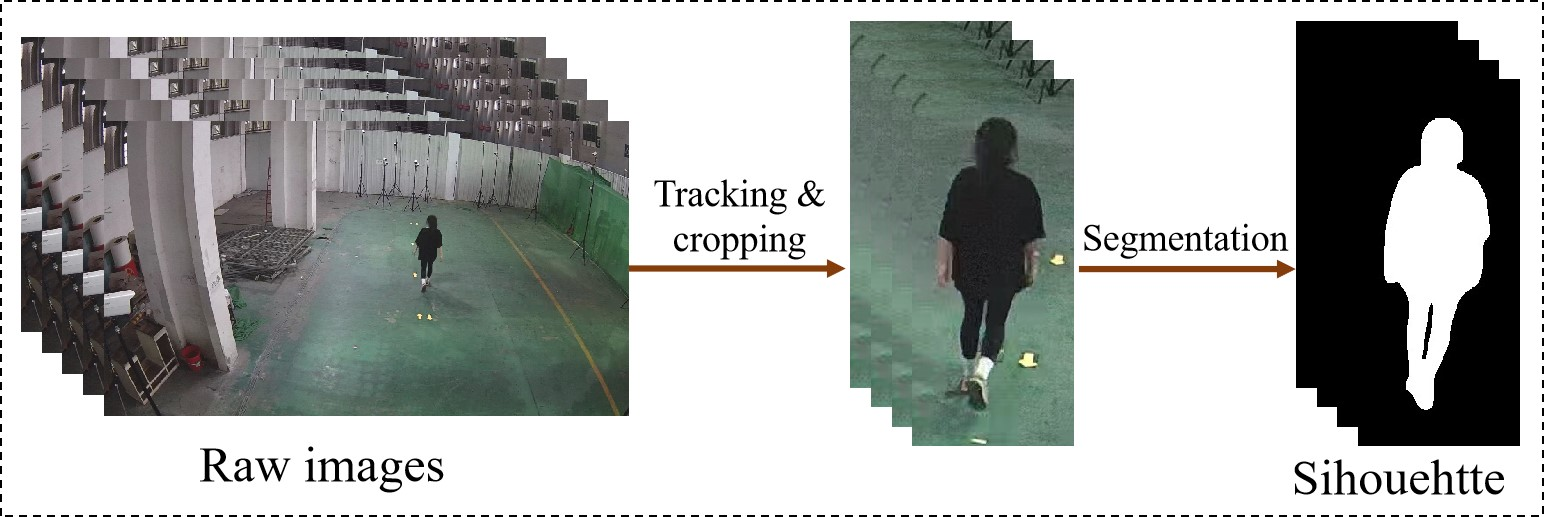
\includegraphics[width=1.0\linewidth]{figures/pre-processing02.jpg}

   \caption{ Pre-processing of D-Gait data generates silhouette images.
   }
   \label{pre-processing}
\end{figure}
\subsection{Data Pre-processing}

After obtaining the raw gait video data, we further pre-process them to prepare the required input data for  deep learning-based depression risk detection methods.
As shown in Fig~\ref{pre-processing}, we first crop the videos with assistance of a multi-object tracking algorithm such that each cropped video clip contains only one walking subject of interests and one gait sequence refers to the video clip of a subject when he/she walks along a straight line towards one direction.
Afterwards,  a real-time instance segmentation algorithm, to obtain the human silhouettes, and then normalize and align the silhouette data.



\subsection{Data cleaning}

The three primary stages of data cleaning are noise removal, frame filtering, and Forward and backward sequence splitting. Below, we'll introduce them one at a time.
(1) Noise removal: During data collection, the camera takes pictures of places that are not being used for data acquisition, such as irrelevant people who are not the subjects.
They should be deleted because they may damage the quality of the data.
(2) Frame filtering: When subjects enter and exit the data collection area, there will be duplicate information, such as changing clothes, as well as an action of turning when subjects reach the end point. Such information is also unwanted and they should be removed.
(3) Forward and backward sequence splitting: During data acquisition, the subjects walk a round trip in the effective area of data acquisition, so there are two image sequences facing the camera or back to the camera, which need to be split and processed.
It takes 10 researchers working for 2 weeks for this tremendous work, and we hope the proposed D-Gait benchmark would facilitate future research of gait depression risk detection.
Note that for privacy concerns, we will first release the pre-processed gait data to the public.


\subsection{Annotations}

To assess the degree of depression of the subjects, we used three internationally used scales, Self-Rating Depression Scale (SDS), Patient Health Questionnaire-9 (PHQ-9), and Generalized Anxiexy Disorde-7 (GAD-7). The subjects were divided into two groups according to their scores: the non-depressed group and the scored depressed group. In order to ensure the validity of the experimental data, we summarized the classification criteria of the scales used in the relevant literature and set the inclusion criteria of the enrolled subjects by combining the specific situation of our data, as described in Table~\ref{scale}.



% Please add the following required packages to your document preamble:
% \usepackage{booktabs}
\begin{table}[]
\caption{The scoring criteria of the selected subjects}
\label{scale}
\setlength{\tabcolsep}{3.5mm}{
\begin{tabular}{@{}c|c|c|c@{}}
\toprule
\textbf{Paper} & \textbf{PHQ-9} & \textbf{SDS} & \textbf{GAD-7} \\ \midrule
Fang~\cite{fang2019depression}  & $score \geq 5$  & $score \geq 50$  & $score \geq 5$             \\
Yang~\cite{yang2022data}        & $score \geq 10$ & $score \geq 60$ & -              \\
Lu~\cite{lu2021new}             & $score \geq 10$ & $score \geq 60$ & -              \\
Wang~\cite{wang2020gait}        & $score \geq 10$ & $score \geq 60$ & -              \\
Daly~\cite{daly2021depression}  & $score \geq 10$ & -      & -              \\
Jing~\cite{jing2019different}   & $score \geq 10$ & -                  & $score \geq 10$       \\
Zhao~\cite{zhao2019see}         & $score \geq 10$ & -      & $score \geq 10$       \\
Choi~\cite{choi2020depression}  & $score \geq 10$ & -      & $score \geq 10$       \\
Hyland~\cite{hyland2020anxiety} & $score \geq 10$ & -      & $score \geq 10$       \\
\textbf{Our}  & $score \geq 10$ & $score \geq 40$ & $score \geq 10$ \\ \bottomrule
\end{tabular}}
\end{table}

The non-depressed group (PHQ-9: mean = 0.92, SD = 1.26; SDS: mean = 6.4, SD = 2.14; GAD-7: mean=0.51, SD=0.95) consisted of 200 individuals
(M: 122, F: 78), whose scores were in the healthy range of both the PHQ-9, SDS, and GAD-7.
The scored-depressed group (PHQ-9: mean = 11.52, SD = 3.24; SDS: mean = 30.52, SD = 6.53; GAD-7: mean=9.40, SD=3.12) contained 200 (M: 92, F: 108) participants.
%The criteria for recruiting the scored-depressed group were that the candidates must be assessed as depression in both the PHQ-9 or SDS.
Candidates for the scored-depressed group had to score depressed on the PHQ-9, SDS, or GAD-7 in order to be included.
In addition, the score had to reach a moderate level in at least one of them ( PHQ-9 score $\geq$ 10 or SDS score $\geq$ 40 or GAD-7 score $\geq$ 10).
Basic information about the subjects is provided in Table~\ref{score}.

% Please add the following required packages to your document preamble:
% \usepackage{booktabs}
\begin{table}[]
\caption{Basic information of the scored-depressed and non-depressed groups.}
\label{score}
\setlength{\tabcolsep}{1mm}{
\begin{tabular}{@{}c|cc@{}}
\toprule
\textbf{ } & \textbf{Scored-depressed} & \textbf{Non-depressed} \\ \midrule
Cases              & 200                       & 200                    \\
Sex (M:F)           & 92:108                    & 122:78                 \\
PHQ-9 ($means \pm SD$) & $11.52 \pm 3.24$          & $0.92 \pm 1.26$              \\
SDS ($means \pm SD$)   & $30.52 \pm 6.53$          & $6.40 \pm 2.14$              \\
GAD-7 ($means \pm SD$) & $9.40 \pm 3.12$           & $0.51 \pm 0.95$              \\ \bottomrule
\end{tabular}}
\end{table}



%%%%%%%%% REFERENCES
{\small
\bibliographystyle{ieee_fullname}
\bibliography{egbib}
}

\end{document}
